\documentclass[11pt]{amsart}
\usepackage{geometry}                % See geometry.pdf to learn the layout options. There are lots.
\geometry{letterpaper}                   % ... or a4paper or a5paper or ... 
%\geometry{landscape}                % Activate for for rotated page geometry
%\usepackage[parfill]{parskip}    % Activate to begin paragraphs with an empty line rather than an indent
\usepackage{algorithmic}
\usepackage{algorithm}
\usepackage{graphicx}
\usepackage{amssymb}
\usepackage{epstopdf}
\DeclareGraphicsRule{.tif}{png}{.png}{`convert #1 `dirname #1`/`basename #1 .tif`.png}

\title{The DBToaster Compilation Algorithm}
\author{Yanif Ahmad, Oliver Kennedy, Christoph Koch}

\newcommand{\todo}[1]{\textcolor{red}{[#1]}}
\newcommand{\note}[1]{\textcolor{blue}{[#1]}}
\newcommand{\tuple}[1]{\left<{#1}\right>}
\newcommand{\parsection}[1]{\smallskip\noindent{\bf #1.}}
\newtheorem{example}{Example}

\renewcommand{\algorithmicrequire}{\textbf{Input:}}
\renewcommand{\algorithmicensure}{\textbf{Output:}}

\begin{document}
\maketitle

\section{Workflow Overview}

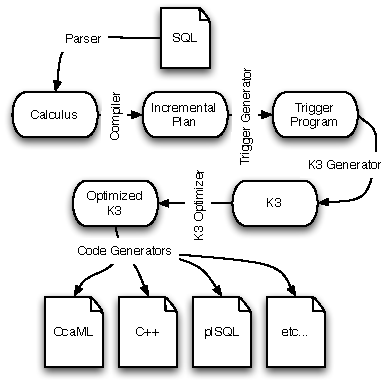
\includegraphics[width=3in]{CompilerFlow}


\section{Calculus}

\begin{verbatim}

type calc_type_t = 
  Int_Type | Double_Type | String_Type

type const_value_t = 
  Integer of int | Double of double | String of string

type var_t = string * calc_type_t

type value_t = 
  Variable of var_t
| Constant of const_value_t

type cmp_t = Lt | Gt | Lte | Gte | Eq | Neq

type calc_t =
  Sum         of calc_t list
  Prod        of calc_t list
  Neg         of calc_t
  AggSum      of var_t list * calc_t
  Value       of value_t
  Relation    of string * var_t list
  Comparison  of value_t * cmp_t * value_t
  Definition  of var_t * calc_t

\end{verbatim}


\section{Incremental Plan (IP)}


\begin{verbatim}

type schema_t = var_t list

type memo_t = 
    string                (* Name *)
    schema_t              (* Schema *)
  * calc_t                (* Defining calculus expression (the calculus 
                             expression that the memo is designed to 
                             maintain/compute *)
  * (   pm_t * string     (* Insert/Delete + Base Relation Name *)
      * map_op_t list     (* Update operations *)
    ) list

and map_op_t =            (* := or += *)
    schema_t              (* target schema mappings *)
  * invocation_t          (* operation *)

and invocation_t =
  * calc_t                (* Calculus expression that the statement invokes *)
  * (                     (* Alternative ways of partitioning the invoked 
                             expression into different memos.  The head of this
                             list is the default approach. *)
        calc_t            (* An expression over zero or more memos that is 
                             semantically equivalent to the invoked expression*)
      * list of memo_t    (* References to memos used by the above expression *)
    ) list

\end{verbatim}

Assertions about the above memo and invocation types (the hypergraph):
\begin{itemize}
\item Initializers initialize the entire Memo, and therefore have no externally bound variables other than the invoked expression's input variables, and the variables which appear in the corresponding initializer.  If an input variable is not bound, it is a loop variable.

\item The access patterns that a Memo is required to support are defined by the set of bound variables in all of its incoming edges.

\item Initializers for memos on the RHS of an expression are stored as part of the calculus expression (External leaves) \footnote{Storing the whole initializer will make working with nonstandard maps (e.g., future work on range trees) difficult.  In effect, the External needs to store a reference to the entire process required to initialize a memo.  On the other hand, this initializer can and should be simplified/compiled given that the set of bound input variables will change.  A reasonable compromise might be to store a list of expressions that the initializer will need to evaluate}.  The LHS memo does not need to be initialized, since the output portion of the memo is guaranteed to be initialized and we'll never see a new input variable in a delta statement.
\end{itemize}

\begin{example}
The following image shows the incremental plan for the query:
$$Q = Sum([], R(a,b) * S(b,c) * T(c,d) * a * d)$$

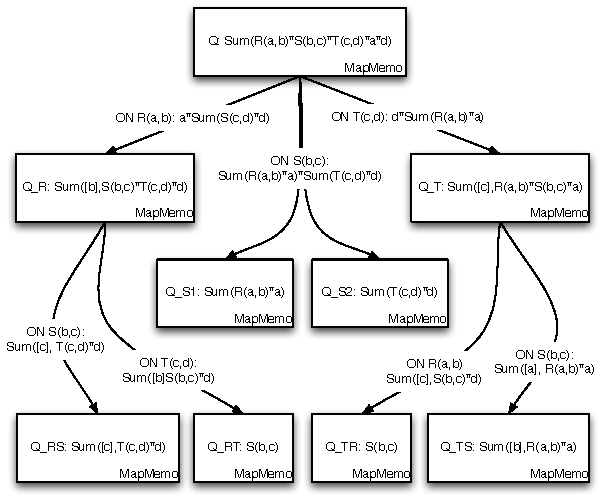
\includegraphics[width=5.5in]{IPExample}
\end{example}

\section{Compilation}

\begin{algorithm}
\caption{compile\_memo (Standard Map)}
\begin{algorithmic}
\REQUIRE{calc\_t $definition$, schema\_t $schema$}
\ENSURE{A memo\_t $memo$}
\STATE Generate a unique name for $memo$
\STATE {\bf calc\_simplify}($definition$)
\FORALL{(Reln,Delta) $(rel, d\_defn) \in$ compute\_deltas($definition$)}
  \STATE {\bf calc\_simplify}($d\_defn$)
  \FORALL{calc\_t $monomial \in d\_defn$}
    \STATE Gather {\bf compile\_invocation}($monomial$)
  \ENDFOR
\ENDFOR
\end{algorithmic}
\end{algorithm}

\begin{algorithm}
\caption{compile\_invocation}
\begin{algorithmic}
\REQUIRE{A monomial calc\_t $expression$}
\ENSURE{An invocation\_t $invocation$}
\STATE Separate the monomial into independent components (i.e., no overlapping internally-bound variables)
\FORALL{Independent calc\_t component $c \in expression$}
  \STATE Pull out all remaining definition terms and create a memo for their RHS.  Then for the remaining terms in the component...
  \STATE (Case 1): Pull out all comparison terms involving input variables and extract a memo for the remaining terms.
  \STATE (Case 2): Create a memo for all the remaining terms
\ENDFOR
\end{algorithmic}
\end{algorithm}

\begin{algorithm}
\caption{calc\_simplify}
\begin{algorithmic}
\REQUIRE{calc\_t $expression$}
\ENSURE{A calc\_t list $monomials$}
\STATE Pull sums in $expression$ up to the top, generating a list of $monomials$
\FORALL{$m \in monomials$}
  \REPEAT
    \STATE {\bf calc\_unify\_vars}($m$)
    \STATE Pull AggSums up and merge where possible
    \STATE Push negation down and merge where possible
    \STATE Move constants left and merge where possible
    \STATE Move comparisons right
    \STATE Eliminate $m$ if it has a 0 or a contradiction (e.g., $(a \theta b) * (a \bar \theta b)$, $(a \neq a)$, $(a < a)$, \ldots)
    \STATE \COMMENT{Some sort of ``lexical" sort might be appropriate}
  \UNTIL{fixedpoint($m$)}
  \STATE Cancel negated sums (e.g., $a + (- a)$)
  \STATE Recurse over subterms of definition terms
\ENDFOR
\STATE 
\end{algorithmic}
\end{algorithm}

\begin{algorithm}
\caption{calc\_unify\_vars}
\begin{algorithmic}
\REQUIRE{a monomial calc\_t $expression$}
\ENSURE{$expression$ with variables unified}
\FORALL{Definition $(v \leftarrow c) \in$ the root level of $expression$}
  \IF{$c$ is a variable bound earlier in the expression, or a constant}
    \STATE replace all occurrences of $v$ in $expression$ with $c$
    \STATE remove the definition ($v \leftarrow c$) from $expression$
  \ENDIF
  \STATE replace all loose (i.e., not in comparison, external, or relation terms) occurrences of $v$ with $c$.
  \IF{$v$ no longer appears in $expression$, or in its parent $AggSum$}
    \STATE remove the definition ($v \leftarrow c$) from $expression$
  \ENDIF
\ENDFOR
\FORALL{Equality Comparison w/ Const $(v = c) \in expression$}
  \STATE Replace $v$ in the expression with $c$
  \STATE remove the comparison ($v = c$) from $expression$
\ENDFOR
\FORALL{Equality Comparison w/ Var $(v_1 = v_2) \in expression$}
  \STATE If possible, replace $v_1$ in the expression with $v_2$ or visa versa
  \STATE remove the comparison ($v_1 = v_2$) from $expression$
\ENDFOR
\end{algorithmic}
\end{algorithm}

\section{Trigger Generation}

The triggers\_for\_X functions translate an Incremental Plan into a set of triggers.  Each trigger is of the form: (1) The Event/Relation name (Variables appearing in the event/relation are drawn from the database schema).  (2) The set of initializers that need to be invoked if necessary (with variables bound as per the schema).  (3) The set of update operations that need to be invoked (with variables bound as per the schema).

\pagebreak
\begin{verbatim}
let trigger_t = 
    string * var_t list                 (* Relation Schema *)
                                        (* Maybe make it a (string * (...))
                                           to make it into an assoc list *)
  * (string * var_t list * calc_t)      (* LHS Initializer *)
  * (string * var_t list * calc_t) list (* Updates *)
\end{verbatim}

\begin{algorithm}
\caption{triggers\_for\_memo}
\begin{algorithmic}
\REQUIRE{memo\_t $memo$}
\ENSURE{A set of gathered initializers and triggers}
\FORALL{Event(Vars) $e(vars) \in memo$}
  \STATE Gather \textbf{triggers\_for\_invocation}($e.initializer$, $e(vars)$)
  \FORALL{Invocation $i \in e.updates$}
    \STATE Gather \textbf{triggers\_for\_invocation}($i$, $e(vars)$)
  \ENDFOR
\ENDFOR
\STATE \textbf{return} gathered triggers
\end{algorithmic}
\end{algorithm}

\begin{algorithm}
\caption{triggers\_for\_invocation}
\begin{algorithmic}
\REQUIRE{invocation\_t $invoc$, (string * var\_t list) $(event, in\_vars)$}
\ENSURE{A set of gathered initializers and triggers}
\STATE Select an implementation $impl \in invoc$
\FORALL{Memo $m \in impl$}
  \STATE Gather \textbf{triggers\_for\_memo}(m)
\ENDFOR
\STATE Add $impl$ to gathered triggers for $event$
\STATE \textbf{return} gathered triggers
\end{algorithmic}
\end{algorithm}

We refer to triggers\_for\_invocation's second parameter as its context.  Context is a way of passing variable bindings through multiple layers of triggers\_for\_invocation, and can contain two types of bindings: (1) Input variables can be bound from above (i.e., as event variables), and (2) Input variables can be bound from the side (i.e., from another map).  

Case 2 only occurs if we have multi-level initializers (i.e., if the initializer for a map reads from a map with an initializer).  In our current design, this is not possible.  Consequently, the algorithm above only handles Case 1.  In order to support Case 2, the following would need to happen:
\begin{itemize}
\item The context needs to be extended to be able to express actual domains (e.g., It needs to be able to express "variables $b$ and $c$ in $M_1[][a,b,c]$").
\item The generated initializer needs to have a way of iterating over the corresponding domain.  This can either be done by applying the above extensions to the datastructure, or by adding in a domain loop like 
$$M_1[a,b][] :=  (dummy \leftarrow M_2[a]) * TheRestOfTheInitializer$$
The former would be preferable, as the latter produces a calculus expression where the input variable is bound from below.
\end{itemize}


\end{document}  